\documentclass{report}
\usepackage{graphicx}
\graphicspath{ {../pictures/} }

\setcounter{secnumdepth}{3}

\setcounter{tocdepth}{3}

\begin{document}

\title{Time Stamper}
\author{Erik Ahlberg}

\maketitle

\tableofcontents

\newpage

\chapter{Introduction}
This document contains the top level description of the Time Stamper application. If you want to get an overall understanding of this project, you are in the right place. The introductory chapters explain the main intent and purpose of this project, painting the broader picture to why things are done the way they are.

The second part dwelves into the business logic of the application. It explains the main services and properties of the application as well as the problem it intends to solve for the customer.

The third and last section of this document describes the overall system design responsible for implementing the desired business logic.

\section{Intent}
The main intent of this project is to acquire new, as well as hone existing, software development skills. It shall ultimately serve its developers in the sense that it is not the end product that is the goal, it is the journey. Each part of the project shall try as far as possible to adhere to the industries best practices, w.r.t. quality and efficiency. The reason is to create a development process and environment that each project member can learn and draw experience from. When the project is over, each member should have acquired a set of new skills and experiences that it can show for in other work related contexts.

\section{Purpose - Business Domain}
Describe the purpose with this project in terms of its business value.

\section{Scope}
Describe the limitations and scope of this project as well as this document.

\chapter{Business Services}
The Time Stamper application is, as the name suggests, a service application for storing time periods for different scenarios. The primary customer is a worker in need for storing the time periods of the working day, e.g. a consultant in the need to record just how much time he/she should bill the customer, see section \ref{section:time_stamping}. In addition, the application stores the data that the client inputs and also has the ability to present it in different ways over time, e.g. a graph of work trends, seasonal differencies etc, see section \ref{section:trends}. Work data submitted over weekly or monthly periods can also result in wage or salary calculation if requested by the Income Calculator service, see section \ref{section:income_calculator}, and last there is also the possibility to save a custom schedule, i.e. the future work schedule used as reference, see section \ref{section:calendar}.

\section{Time Stamping}
\label{section:time_stamping}
One of the main services of the application, the time stamping functionality, is used to register the time periods of the client. The user interface of the service is illustrated in figure \ref{figure:time_stamping_activity}. At the centre is the stamping button which is the communication interface for the client to store start- and end times of an arbitrary period.

\begin{figure}
\centering
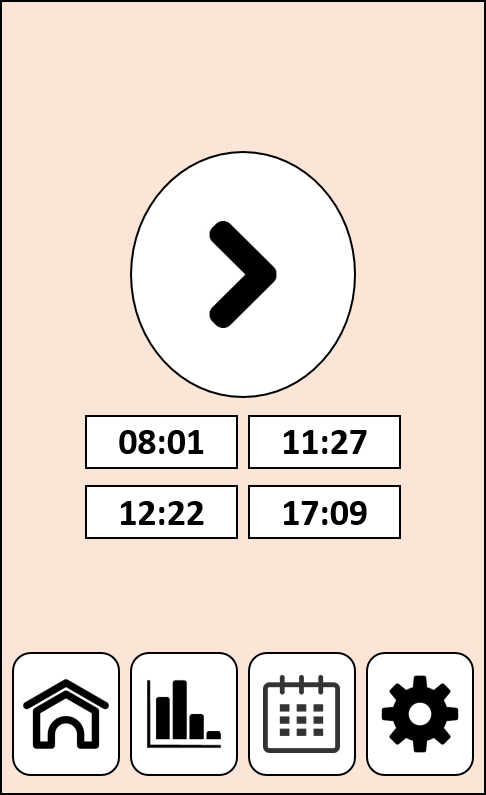
\includegraphics[width=0.3\linewidth]{time_stamping_activity.png}
\caption{The Time Stamping user interface.}
\label{figure:time_stamping_activity}
\end{figure}

Each registered period, consisting of a start- and end time, is automatically shown in the respective fields below the button. There can be an arbitrary number of time periods registered, but they are limited to a 24 hour period. Once the period is over, the time stamp period is registered for the subsequent 24 hour period.

\section{Trends}
\label{section:trends}

\begin{figure}
\centering
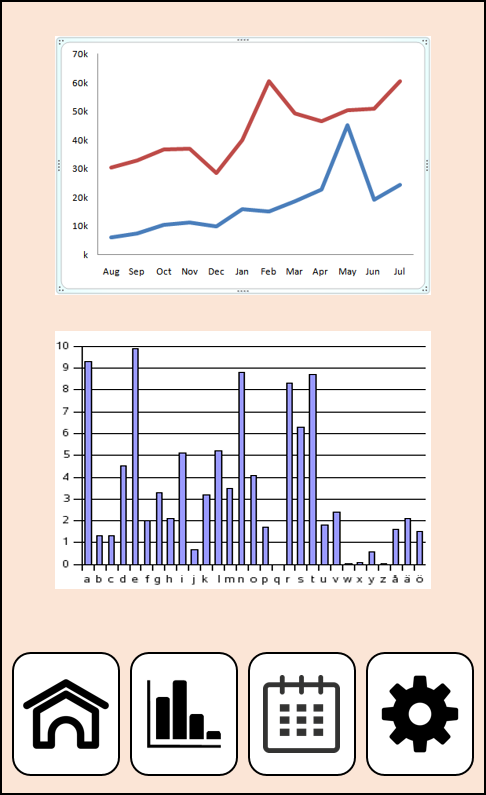
\includegraphics[width=0.3\linewidth]{trends_activity.png}
\caption{The Trends user interface.}
\label{figure:trends_activity}
\end{figure}

The time period data the client stores can and will be used to show the user his/her trends and patterns. For instance, depending on the usage of the application, both in frequency and time, it can present the complete time periods over the current week, month or year. Compare time periods between years and calculate averages over custom periods. These services are available under the Trends activity user interface, see figure \ref{figure:trends_activity}, and operate directly on the stored client data.

\section{Calendar}
\label{section:calendar}

\begin{figure}
\centering
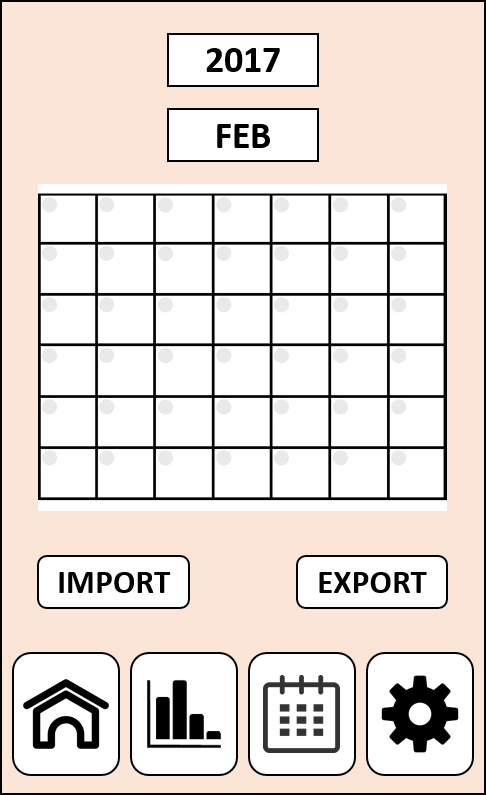
\includegraphics[width=0.3\linewidth]{calendar_activity.png}
\caption{The Calendar user interface.}
\label{figure:calendar_activity}
\end{figure}

The calender is used to visualize the already time stamped periods on a date basis and also to visualize a pre-loaded schedule for future usage. The pre-loaded schedule shall at least be compatible with the Microsoft Outlook format and/or Google Calendar so any existing schedules from these formats can easily be migrated. Also, if requested, the calender, both stored time periods and loaded future schedules, can be exported to any of the above mentioned formats. The calendar service is available under the Calendar activity shown in figure \ref{figure:calendar_activity}.

\section{Income Calculator}
\label{section:income_calculator}
Description of the income calculator function.

\chapter{System Design}
Overall summary of the total system meant to produce the previously described business services.

\section{System Architecture}
Overall summary of the system components that comprise the complete architecture for the system.

\subsection{System Components}
In detail description of the components comprising the complete system, and their roles within it.

\subsubsection{Component Interactions}
In detail descritpion of the component interactions, i.e. their communication patterns, with each other.

\subsection{Client Front-End}
In detail description of the front-end applicaiton.

\subsection{Back-End Services}
In detail description of the back-end application.

\chapter{System Requirements}
Collection of necessary system requirements.

\end{document}

